% Cole Nielsen niels538@umn.edu
% EE 2002 Spring 2015
% Formal Lab Report 1

%----------------------------------------------------------------------------------------
%	PACKAGES AND DOCUMENT CONFIGURATIONS
%----------------------------------------------------------------------------------------

\documentclass[12pt]{article}

\usepackage{circuitikz}
\usepackage{graphicx}
\usepackage{subcaption}
\usepackage[top=1in, bottom= 1in, left=1in, right= 1in]{geometry}
\setlength\parindent{0pt}
\usepackage{fancyhdr}
\pagestyle{fancy}
\usepackage{textcomp}
\usepackage{tikz}
\usepackage{siunitx}
\usepackage{placeins}
\usepackage{titlesec}
\usepackage{cancel} 
\ctikzset{tripoles/mos style/arrows}
\tikzset{srail/.style={sground,yscale=-1}}
%----------------------------------------------------------------------------------------
%	DOCUMENT INFORMATION
%----------------------------------------------------------------------------------------

\title{Experiment N\textsuperscript{\underline{o}} 5:   \\ High-Frequency Behavior\\ of
MOSFETs\\ \vspace{0.3 in} EE 3101}

\author{Cole \textsc{Nielsen}} 
\date{Fall 2015}

\newcommand{\mymeter}[2]{   	% #1 = name , #2 = rotation angle
 \begin{scope}[transform shape,rotate=#2]
   \draw[thick] (#1)node(){$\mathbf V$} circle (11pt);
   \draw[rotate=45,-latex] (#1)  +(-17pt,0) --+(17pt,0);
 \end{scope}
}

\begin{document}
\maketitle 

\begin{center}
 \begin{tabular}{l r}
   Dates Performed: & Nov. 11 \& 18, 2015 \\ 
   Instructor: & Kyle Fox \\ 
\end{tabular}
\end{center}
\pagebreak
%----------------------------------------------------------------------------------------
%	Abstract
%----------------------------------------------------------------------------------------
\begin{abstract}
\noindent 
The small signal behavior and frequency response of several MOSFET amplifiers was tested in this experiment. The tendency of a common source (CS) amplifier to pass a midband with gain $g_m$ was observed. By varying the drain resistance of the amplifier and observing the change in cutoff frequency, the gate to drain and gate to source capacitances of a 2N7000 MOSFET was determined. A cascode amplifier and Common-Drain-Common-Gate (CD-CG) amplifier were then built and the midband gain and bandwidth of each circuit was found. It was determined for the same bias current and transistors, a CD-CG amplifier has the greatest bandwidth, followed by the cascode amplifier, and the CS amplifier had the worst performance.
\end{abstract}
\hrulefill
%----------------------------------------------------------------------------------------
%	Introduction
%----------------------------------------------------------------------------------------
\section{Introduction}
%
Principle to the study of electrical engineering is the amplification of signals. Amplification is simply the process of increasing the power of a signal, and it is of interest because it allows us to take small signals, like that from a microphone or some other sensor, and boost them to drive large loads like speakers. Another example is in digital radio communications, where low power signals are generated in digital processors, and then amplifier circuits are used to amplify those signals greatly so they can be transmitted long distances. Many approaches have been devised to amplify signals, using tube and transistor based technologies. This experiment focused on the use of MOSFETs (Metal-Oxide-Semiconductor Field-Effect-Transistor) to provide voltage gain of an input voltage signal. The MOSFET in basic acts as a transconductance amplifier, where a voltage applied to the gate (relative to source) will result in a current to flow from drain to source when some voltage is present. Quantitatively, this relationship is given as follows:
\begin{equation}
I_d = \frac{1}{2} k_n^`\Big(\frac{W}{L}\Big)V_{ov}^2
\label{eq:wan}
\end{equation}
Where $k_n^`\Big(\frac{W}{L}\Big)$ are process-specific parameters for channel size and transconductance, and $V_{ov}$ is the voltage of $V_{gs}$ over the threshold voltage. Note this relationship is non-linear. This has a couple implications, one being MOSFET amplifiers will inherently distort signals, and another is that the exact behavior of MOSFETs cannot be modeled easily using traditional linear methods. To work around this, the small signal model is used to provide a linearization of MOSFET behavior for AC signals. The small signal model assumes an amplifier will be biased with some quiescent DC voltage at the gate, resulting in a DC current $I_d$. It can be assumed that for a small change in gate voltage, the change in current can be estimated using the linearization of the I-V curve at the original DC operating point. This linearization can simply be found via differentiation of equation \ref{eq:wan}, which yields:
\begin{equation}
g_m = \frac{2I_d}{V_{ov}}
\end{equation}
Where $g_m$ is the small signal transconductance, and is the slope of the MOSFET I-V curve for $I_d$. It is important to know that this linearization is only accurate near the bias point, so  signals with small variations from this point (hence the small signal model) must be used to reasonably model amplifier behaviors. If some resistor is used to load the MOSFET, and a some small signal $v_{gs}$ is applied to the gate, it is expected that the resulting current should be $g_mv_{gs}$, and thus the change of voltage across the resistor should be $iR = g_mv_{gs}R$. If this voltage is taken to be the output voltage, the gain of the amplifier is then $\frac{v_o}{v_{gs}}=\pm g_mR$ depending on the topology. This is the basic principle of the MOSFET amplifier.\\\par

The basic small signal model just assumes that the MOSFET is a a dependent current source, controlled by the gate to source voltage, and that the gate is floating. In real life, however, capacitors are formed by the physical structures of MOSFET transistors between the gate and drain and the gate and source. This complicates the behavior of the small signal model, as when resistors are added, RC filters are formed with the transistor. This causes the gain to be a function of frequency, practically limiting how high and low frequency an amplifier can operate. The band that an amplifier can operate in is called the mid band, and has an associated bandwidth and gain. Understanding this particular behavior of actual transistors will be the focus of this lab, and will be done first by testing a common-source (CS) amplifier to determine its frequency dependent behaviour. From experimental data with the CS amplifier, the size of the gate-source and gate-drain capacitances of a 2N7000 MOSFET will be calculated. Then cascode and CD-CG amplifiers will be designed and tested to determine which topology offers the best performance in terms of bandwidth and gain to minimize the effects of gate capacitance.
%----------------------------------------------------------------------------------------
%	Experiment
%----------------------------------------------------------------------------------------
\section{Experiment}
\subsection*{Part 1 - Common Source Amplifier}
The common-source amplifier shown below was designed with $V_{DD}$ = 16 V, $V_{DS}$ = 8 V, $I_D$ = 2 mA, $R_g$ = 5 k$\Omega$, $R_S$ = $R_D$, and that the capacitors $C_G$ and $C_S$ appear to have low impedance relative to the input impedance at 1 kHz. The transconductance at midband frequencies and midband gain was found for this amplifier theoretically and experimentally.
\FloatBarrier
\begin{figure}[h!]
\begin{center}
 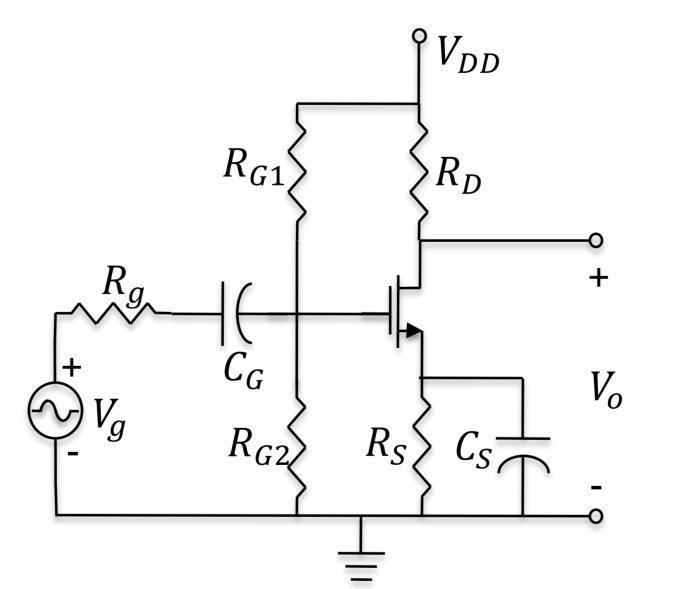
\includegraphics[scale=0.23]{./plots/1.png}
\end{center}
\caption{CS Amplifier}
\end{figure}
\FloatBarrier
\textbf{Calculations}\\
If $V_{DD}$ = 16 V, $V_{DS}$ = 8 V, and $R_S$ = $R_D$, we should expect $V_{RD}$ = $V_{RS}$ = 4 V. $I_D$ is required to be 2 mA, so  
\begin{equation}
R_S = R_D = \frac{4}{0.002} = 2 k\Omega
\end{equation}
A 2N7000 was quick set up with 8V across drain to source, with a DMM measuring current and a potentiometer to adjust gate voltage. By sweeping the gate voltage and observing the current, it was found that $V_{gs}$ for 2 mA was 2.333 volts, and from the datasheet $V_t$ is reported to be 2.1 V, therefore $V_{ov}$ is $V_{gs}$ - $V_t$ = 0.233 V for 2 mA. $g_m$ is predicted to be as follows:
\begin{equation}
g_m = \frac{2I_D}{V_{ov}} = \frac{2\times 0.002}{0.233} = 0.01716\hspace{6pt} \frac{A}{V}
\end{equation}
To calculate $R_{G1}$ and $R_{G2}$, $V_{g}$ is first noted to be $V_{gs}$ + $V_{RS}$ = 6.333 V. Calculating the voltage divider formed by the two resistors, and choosing $R_{G2}$ = 1 M$\Omega$ (to ensure high input Z), $R_{G1}$ is found to be:
\begin{equation}
\frac{V_o}{V_i} = \frac{R_{G2}}{R_{G1}+R_{G2}} \rightarrow 16 = 6.33 \frac{1M}{R_{G1} + 1M}\rightarrow R_{G1} \approx 1.5 M\Omega
\end{equation}
$C_G$ and $C_S$ were arbitrarily chosen to be 10$\mu$F, which leads to a $X_C$ = 15.9 $\Omega$, which is far less then the 0.6 M$\Omega$ $R_{in}$\\

Finally, $g_m$ can be calculated experimentally as $V_o$ = $-g_m v_{gs} R_D$, and $v_{gs} \approx V_i$, so $g_m = \frac{-V_o}{V_i R_D}$\\\par

\textbf{Experiment}\\
The circuit was breadboarded as designed, and a function generator was connected to the input of the circuit. An oscilloscope was then used to probe the input and output of the circuit with 10X probes. A 78.4 mV input sinusoid was then swept from 1 kHz to 70 KHz, and the signal amplitude was recorded at various frequencies in between.\\\par
\textbf{Data}\\The recorded values for $V_o$ were used to calculate $g_m$ for various frequencies, and then were plotted against log scale frequency. The maximal (midband) transconductance was observed to be 0.0134, corresponding to a gain of 26.8.
\FloatBarrier
\begin{figure}[h!]
\begin{center}
    	\resizebox{0.6\textwidth}{!}{% GNUPLOT: LaTeX picture
\setlength{\unitlength}{0.240900pt}
\ifx\plotpoint\undefined\newsavebox{\plotpoint}\fi
\sbox{\plotpoint}{\rule[-0.200pt]{0.400pt}{0.400pt}}%
\begin{picture}(1500,900)(0,0)
\sbox{\plotpoint}{\rule[-0.200pt]{0.400pt}{0.400pt}}%
\put(211.0,131.0){\rule[-0.200pt]{4.818pt}{0.400pt}}
\put(191,131){\makebox(0,0)[r]{ 0.008}}
\put(1419.0,131.0){\rule[-0.200pt]{4.818pt}{0.400pt}}
\put(211.0,239.0){\rule[-0.200pt]{4.818pt}{0.400pt}}
\put(191,239){\makebox(0,0)[r]{ 0.009}}
\put(1419.0,239.0){\rule[-0.200pt]{4.818pt}{0.400pt}}
\put(211.0,346.0){\rule[-0.200pt]{4.818pt}{0.400pt}}
\put(191,346){\makebox(0,0)[r]{ 0.01}}
\put(1419.0,346.0){\rule[-0.200pt]{4.818pt}{0.400pt}}
\put(211.0,454.0){\rule[-0.200pt]{4.818pt}{0.400pt}}
\put(191,454){\makebox(0,0)[r]{ 0.011}}
\put(1419.0,454.0){\rule[-0.200pt]{4.818pt}{0.400pt}}
\put(211.0,561.0){\rule[-0.200pt]{4.818pt}{0.400pt}}
\put(191,561){\makebox(0,0)[r]{ 0.012}}
\put(1419.0,561.0){\rule[-0.200pt]{4.818pt}{0.400pt}}
\put(211.0,669.0){\rule[-0.200pt]{4.818pt}{0.400pt}}
\put(191,669){\makebox(0,0)[r]{ 0.013}}
\put(1419.0,669.0){\rule[-0.200pt]{4.818pt}{0.400pt}}
\put(211.0,776.0){\rule[-0.200pt]{4.818pt}{0.400pt}}
\put(191,776){\makebox(0,0)[r]{ 0.014}}
\put(1419.0,776.0){\rule[-0.200pt]{4.818pt}{0.400pt}}
\put(211.0,131.0){\rule[-0.200pt]{0.400pt}{2.409pt}}
\put(211.0,766.0){\rule[-0.200pt]{0.400pt}{2.409pt}}
\put(272.0,131.0){\rule[-0.200pt]{0.400pt}{2.409pt}}
\put(272.0,766.0){\rule[-0.200pt]{0.400pt}{2.409pt}}
\put(319.0,131.0){\rule[-0.200pt]{0.400pt}{2.409pt}}
\put(319.0,766.0){\rule[-0.200pt]{0.400pt}{2.409pt}}
\put(358.0,131.0){\rule[-0.200pt]{0.400pt}{2.409pt}}
\put(358.0,766.0){\rule[-0.200pt]{0.400pt}{2.409pt}}
\put(390.0,131.0){\rule[-0.200pt]{0.400pt}{2.409pt}}
\put(390.0,766.0){\rule[-0.200pt]{0.400pt}{2.409pt}}
\put(418.0,131.0){\rule[-0.200pt]{0.400pt}{2.409pt}}
\put(418.0,766.0){\rule[-0.200pt]{0.400pt}{2.409pt}}
\put(443.0,131.0){\rule[-0.200pt]{0.400pt}{2.409pt}}
\put(443.0,766.0){\rule[-0.200pt]{0.400pt}{2.409pt}}
\put(466.0,131.0){\rule[-0.200pt]{0.400pt}{4.818pt}}
\put(466,90){\makebox(0,0){ $10^3$}}
\put(466.0,756.0){\rule[-0.200pt]{0.400pt}{4.818pt}}
\put(612.0,131.0){\rule[-0.200pt]{0.400pt}{2.409pt}}
\put(612.0,766.0){\rule[-0.200pt]{0.400pt}{2.409pt}}
\put(698.0,131.0){\rule[-0.200pt]{0.400pt}{2.409pt}}
\put(698.0,766.0){\rule[-0.200pt]{0.400pt}{2.409pt}}
\put(759.0,131.0){\rule[-0.200pt]{0.400pt}{2.409pt}}
\put(759.0,766.0){\rule[-0.200pt]{0.400pt}{2.409pt}}
\put(806.0,131.0){\rule[-0.200pt]{0.400pt}{2.409pt}}
\put(806.0,766.0){\rule[-0.200pt]{0.400pt}{2.409pt}}
\put(844.0,131.0){\rule[-0.200pt]{0.400pt}{2.409pt}}
\put(844.0,766.0){\rule[-0.200pt]{0.400pt}{2.409pt}}
\put(877.0,131.0){\rule[-0.200pt]{0.400pt}{2.409pt}}
\put(877.0,766.0){\rule[-0.200pt]{0.400pt}{2.409pt}}
\put(905.0,131.0){\rule[-0.200pt]{0.400pt}{2.409pt}}
\put(905.0,766.0){\rule[-0.200pt]{0.400pt}{2.409pt}}
\put(930.0,131.0){\rule[-0.200pt]{0.400pt}{2.409pt}}
\put(930.0,766.0){\rule[-0.200pt]{0.400pt}{2.409pt}}
\put(952.0,131.0){\rule[-0.200pt]{0.400pt}{4.818pt}}
\put(952,90){\makebox(0,0){ $10^4$}}
\put(952.0,756.0){\rule[-0.200pt]{0.400pt}{4.818pt}}
\put(1099.0,131.0){\rule[-0.200pt]{0.400pt}{2.409pt}}
\put(1099.0,766.0){\rule[-0.200pt]{0.400pt}{2.409pt}}
\put(1184.0,131.0){\rule[-0.200pt]{0.400pt}{2.409pt}}
\put(1184.0,766.0){\rule[-0.200pt]{0.400pt}{2.409pt}}
\put(1245.0,131.0){\rule[-0.200pt]{0.400pt}{2.409pt}}
\put(1245.0,766.0){\rule[-0.200pt]{0.400pt}{2.409pt}}
\put(1292.0,131.0){\rule[-0.200pt]{0.400pt}{2.409pt}}
\put(1292.0,766.0){\rule[-0.200pt]{0.400pt}{2.409pt}}
\put(1331.0,131.0){\rule[-0.200pt]{0.400pt}{2.409pt}}
\put(1331.0,766.0){\rule[-0.200pt]{0.400pt}{2.409pt}}
\put(1364.0,131.0){\rule[-0.200pt]{0.400pt}{2.409pt}}
\put(1364.0,766.0){\rule[-0.200pt]{0.400pt}{2.409pt}}
\put(1392.0,131.0){\rule[-0.200pt]{0.400pt}{2.409pt}}
\put(1392.0,766.0){\rule[-0.200pt]{0.400pt}{2.409pt}}
\put(1417.0,131.0){\rule[-0.200pt]{0.400pt}{2.409pt}}
\put(1417.0,766.0){\rule[-0.200pt]{0.400pt}{2.409pt}}
\put(1439.0,131.0){\rule[-0.200pt]{0.400pt}{4.818pt}}
\put(1439,90){\makebox(0,0){ $10^5$}}
\put(1439.0,756.0){\rule[-0.200pt]{0.400pt}{4.818pt}}
\put(211.0,131.0){\rule[-0.200pt]{0.400pt}{155.380pt}}
\put(211.0,131.0){\rule[-0.200pt]{295.825pt}{0.400pt}}
\put(1439.0,131.0){\rule[-0.200pt]{0.400pt}{155.380pt}}
\put(211.0,776.0){\rule[-0.200pt]{295.825pt}{0.400pt}}
\put(30,453){\makebox(0,0){\hspace{-108pt}Transconductance ($g_m$)}}
\put(825,29){\makebox(0,0){Frequency (Hz)}}
\put(825,838){\makebox(0,0){Common Source Amplifier $g_m$ vs Frequency}}
\put(466,668){\usebox{\plotpoint}}
\multiput(466.00,668.58)(3.890,0.498){85}{\rule{3.191pt}{0.120pt}}
\multiput(466.00,667.17)(333.377,44.000){2}{\rule{1.595pt}{0.400pt}}
\multiput(1099.00,710.92)(1.668,-0.498){85}{\rule{1.427pt}{0.120pt}}
\multiput(1099.00,711.17)(143.038,-44.000){2}{\rule{0.714pt}{0.400pt}}
\multiput(1245.58,664.90)(0.499,-0.809){169}{\rule{0.120pt}{0.747pt}}
\multiput(1244.17,666.45)(86.000,-137.451){2}{\rule{0.400pt}{0.373pt}}
\multiput(1331.58,516.16)(0.497,-3.777){63}{\rule{0.120pt}{3.094pt}}
\multiput(1330.17,522.58)(33.000,-240.578){2}{\rule{0.400pt}{1.547pt}}
\put(806.0,712.0){\rule[-0.200pt]{70.584pt}{0.400pt}}
\put(466,668){\rule{1pt}{1pt}}
\put(806,712){\rule{1pt}{1pt}}
\put(952,712){\rule{1pt}{1pt}}
\put(1099,712){\rule{1pt}{1pt}}
\put(1245,668){\rule{1pt}{1pt}}
\put(1331,529){\rule{1pt}{1pt}}
\put(1364,282){\rule{1pt}{1pt}}
\put(211.0,131.0){\rule[-0.200pt]{0.400pt}{155.380pt}}
\put(211.0,131.0){\rule[-0.200pt]{295.825pt}{0.400pt}}
\put(1439.0,131.0){\rule[-0.200pt]{0.400pt}{155.380pt}}
\put(211.0,776.0){\rule[-0.200pt]{295.825pt}{0.400pt}}
\end{picture}
}
\end{center}
\caption{CS Amplifier Transconductance Frequency Response}
\caption*{Midband $g_m$ = 0.0134}
\end{figure}
\FloatBarrier
\textbf{Conclusions}\\
The amplifier behaved closely as designed, having a transconductance of 0.0134, which is 22\% lower than the predicted 0.01716. This is lower than expected, and is likely due to biasing being off from ideal values, and that the threshold voltage is possibly different than the 2.1 V given by the datasheet. It was also observed that the transconductance exhibited a dependence on frequency, dropping off with increases in frequency. This implies that this amplifier is limited as to how high of a frequency it can amplify to. This effect is a result of gate capacitances in the transistor forming RC filters in the amplifier, and making the gain of amplifier dependent on frequency. 
\subsection*{Part 2- Common Source Amplifier Cutoff Frequency}
Using the circuit of the previous part, the cut off frequency of the amplifier was determined as the point where the gain dropped to half power (-3 dB) from the midband gain.\\\par
\textbf{Calculations}\\
The midband gain of the circuit of part one was found to be 26.8, so the half power point is will be when $g_m$ = $\frac{26.8}{\sqrt{2}}= 18.9$, or when the output voltage amplitude is $\frac{1}{\sqrt{2}}$ times that of the maximal amplitude\\\par
\textbf{Experiment}\\
The same circuit and set up was used as part one. The frequency was first swept to determine the maximal voltage of the amplifier (midband value), and then the cut off amplitude was then calculated from that value. The frequency was then swept until the frequency that corresponded to the half power was found.\\\par 
\textbf{Data/Conclusions}\\
It was found experimentally that the half power (cutoff) frequency for the CS amplifier occured at 72 kHz. This was the upper cutoff of the mid band, after which the amplitude falls off like a low pass filter.
\subsection*{Part 3- Modified CS Amplifier Cutoff}
The circuit of part one was modified such that the value of $R_D$ was cut in half, with the intent to change the frequency response of the circuit. From the two different values for cutoff in this circuit at different $R_D$ values, the size of the gate to drain capacitance ($C_{gd}$) and the gate to source capacitance ($C_{gs}$) will be found in the following part.\\\par
\textbf{Experiment}\\
The same circuit and set up was used as part one. The frequency was first swept to determine the maximal voltage of the amplifier (midband value), and then the cut off amplitude was then calculated from that value. The frequency was then swept until the frequency that corresponded to the half power was found.\\\par
\textbf{Data/Conclusion}\\
Experimentally it was found $f_H$ = 145 kHz for a halved $R_D$. This is value is double the original, which makes sense, as a RC cutoff typically is calculated as $\frac{1}{RC}$, and by cutting R in half would lead to a doubling in frequency.

\subsection*{Part 4- MOSFET C$_\textnormal{gd}$ and C$_\textnormal{gs}$ Calculation}
From the using the previously found two cutoff frequencies for different $R_D$ values, the size of the gate to drain capacitance ($C_{gd}$) and the gate to source capacitance ($C_{gs}$) will be found. These capacitances are modeled like below in the shown MOSFET small signal model:\\\par
\FloatBarrier
\begin{figure}[h!]
\begin{center}
 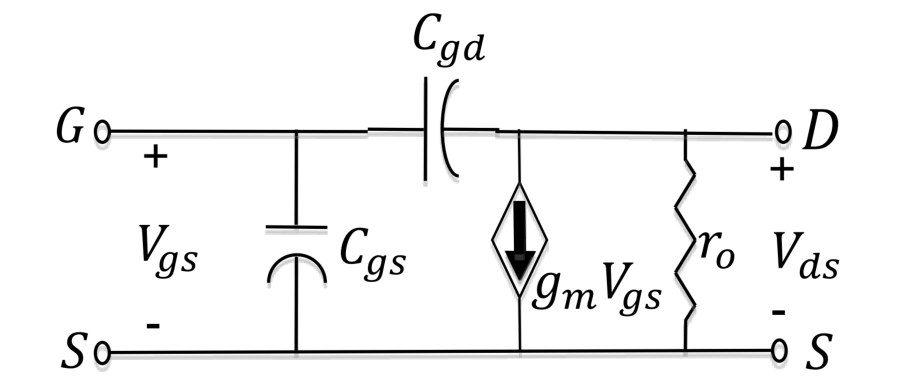
\includegraphics[scale=0.23]{./plots/3.png}
\end{center}
\caption{Small Signal Model with Gate Capacitances}
\end{figure}
\FloatBarrier
Using the Miller effect the cutoff frequency for the CS amplifier can be approximated as:
\begin{equation}
\frac{1}{2\pi(R_G || R_{G_1} || R_{G_2})[C_{gs} + C_{gd}(1 + g_m R_d)] }
\end{equation}
\textbf{Calculations}\\
Applying the Miller Effect cutoff frequency equation for the CS amplifier, the two sets of data for $R_D$ and $f_H$ can be plugged in to result in two simultaneous equations that can be solved for $C_{gs}$ and $C_{gd}$. Doing so leads to :
\begin{equation}
72k = \frac{1}{2\pi(5k || 1M || 1.5M)[C_{gs} + C_{gd}(1 + 0.0134 \times 2000)] }
\end{equation}
\begin{equation}
145k = \frac{1}{2\pi(5k || 1M || 1.5M)[C_{gs} + C_{gd}(1 + 0.0134 \times 1000)] }
\end{equation}
\\\par
Solving these for $C_{gs}$ and $C_{gd}$ gives $C_{gs}$ = -19.9 pF and $C_{gd}$ = 16.8 pF.\\\par
\textbf{Conclusion}\\
The values for $C_{gs}$ and $C_{gd}$ were shown to be non-trivial here, having values in the order of tens of picofarads. These values seem to agree with the values provided in the Fairchild data sheet, which cited a typical input capacitance as 20 pF, which is very close to the measured values. The value for $C_{gs}$ solved out to be negative, however, which is possibly due to limitations of the approximations made throughout the experiment. As seen by the previous sections, the effects of these capacitances where such that they limited the frequency of which the amplifiers could operate, which limits their utility. Fortunately applying and understanding the Miller effect can help to overcome the limitations  by these capacitances. A general way to increase bandwidth in a CS topology is to minimize the resistances used, possibly by driving the amplifier with preceding stage with low output resistance, allowing for $R_{in}$ to be low, or by having a low impedance load on the output.
\subsection*{Part 5- Cascode Amplifier}
The objective of this part is to design a cascode Amplifier, shown below, to improve upon the bandwidth of the CS amplifier. The bias points should remain the same in the circuit as the CS amplifier. The bandwidth and gain should then be measured.
\FloatBarrier
\begin{figure}[h!]
\begin{center}
 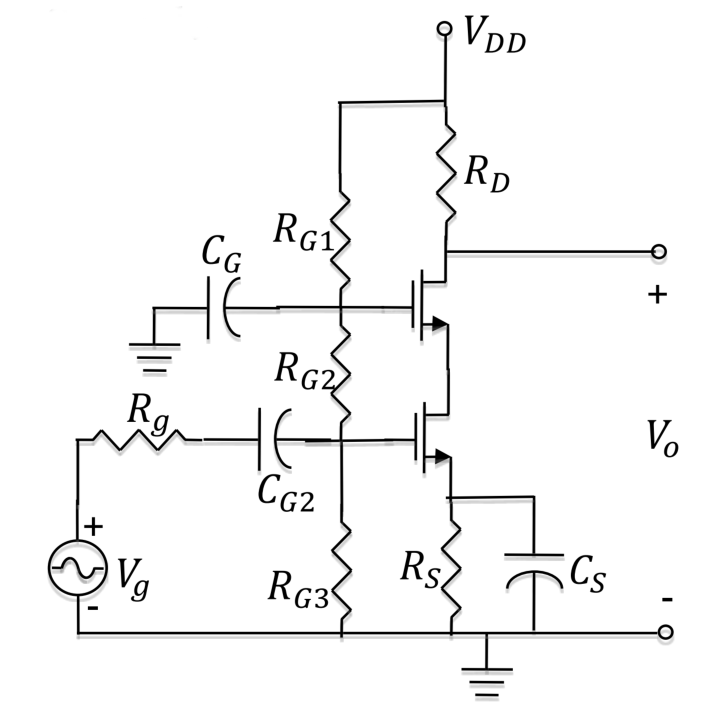
\includegraphics[scale=0.23]{./plots/5.png}
\end{center}
\caption{Cascode Amplifier}
\end{figure}
\FloatBarrier
\textbf{Calculations}\\
All of the Component values should remain the same, except for the resistors to set the DC bias values on the transistor gates. These should be set such that the drain current is 2 mA, or $V_{gs}$ = 2.333 V. The voltage of the lower transistor's gate should be set to $V_{g2}$ = $V_{RS}$ + $V_{gs}$ = 4 + 2.333 = 6.333 V. The second gate should be set to $V_{g2}$ = $V_{RS}$ + $V_{DS}$ + $V_{gs}$ = 4 + 2 + 10.333 V. This can be solved for using voltage divider equations. $R_{G2}$ will be assumed to be 1 M$\Omega$.
\begin{equation}
V_{G1} = V_{DD}\frac{R_{G2}+R_{G3}}{R_{G1} + R_{G2}+R_{G3}} \rightarrow 10.333 = 16\frac{1M+R_{G3}}{R_{G1} + 1M+R_{G3}}
\end{equation}
\begin{equation}
V_{G2} = V_{DD}\frac{R_{G3}}{R_{G1} + R_{G2}+R_{G3}} \rightarrow 6.333 = 16\frac{R_{G3}}{R_{G1} + 1M+R_{G3}}
\end{equation}
Solving the two equations for $R_{G1}$ and $R_{G3}$ gives $R_{G1}$ = 1.42 M$\Omega$ and $R_{G3}$ = 1.58 M$\Omega$.
\textbf{Experiment}\\
The circuit was breadboarded as designed, and a function generator was connected to the input of the circuit. An oscilloscope was then used to monitor the input and output of the circuit with 10X probes. The input was held at approximately 114 mV, and the frequency was swept from 100 Hz to 1 MHz, hitting in intervals of 100, 300, 1k, 3k and so on for even log spacing for frequency. The values for amplitude were recorded, and the cutoffs determined.\\\par
\textbf{Data}\\ Gain was determined as the ratio of output voltage to input at each measured frequency, and then was plotted with log frequency scaling. A dotted line representing half power gain is included, as well as numerical values for cutoffs and midband gain.
\FloatBarrier
\begin{figure}[h!]
\begin{center}
    	\resizebox{0.6\textwidth}{!}{% GNUPLOT: LaTeX picture
\setlength{\unitlength}{0.240900pt}
\ifx\plotpoint\undefined\newsavebox{\plotpoint}\fi
\begin{picture}(1500,900)(0,0)
\sbox{\plotpoint}{\rule[-0.200pt]{0.400pt}{0.400pt}}%
\put(151.0,131.0){\rule[-0.200pt]{4.818pt}{0.400pt}}
\put(131,131){\makebox(0,0)[r]{ 10}}
\put(1419.0,131.0){\rule[-0.200pt]{4.818pt}{0.400pt}}
\put(151.0,292.0){\rule[-0.200pt]{4.818pt}{0.400pt}}
\put(131,292){\makebox(0,0)[r]{ 15}}
\put(1419.0,292.0){\rule[-0.200pt]{4.818pt}{0.400pt}}
\put(151.0,454.0){\rule[-0.200pt]{4.818pt}{0.400pt}}
\put(131,454){\makebox(0,0)[r]{ 20}}
\put(1419.0,454.0){\rule[-0.200pt]{4.818pt}{0.400pt}}
\put(151.0,615.0){\rule[-0.200pt]{4.818pt}{0.400pt}}
\put(131,615){\makebox(0,0)[r]{ 25}}
\put(1419.0,615.0){\rule[-0.200pt]{4.818pt}{0.400pt}}
\put(151.0,776.0){\rule[-0.200pt]{4.818pt}{0.400pt}}
\put(131,776){\makebox(0,0)[r]{ 30}}
\put(1419.0,776.0){\rule[-0.200pt]{4.818pt}{0.400pt}}
\put(151.0,131.0){\rule[-0.200pt]{0.400pt}{4.818pt}}
\put(151,90){\makebox(0,0){ $10^2$}}
\put(151.0,756.0){\rule[-0.200pt]{0.400pt}{4.818pt}}
\put(248.0,131.0){\rule[-0.200pt]{0.400pt}{2.409pt}}
\put(248.0,766.0){\rule[-0.200pt]{0.400pt}{2.409pt}}
\put(305.0,131.0){\rule[-0.200pt]{0.400pt}{2.409pt}}
\put(305.0,766.0){\rule[-0.200pt]{0.400pt}{2.409pt}}
\put(345.0,131.0){\rule[-0.200pt]{0.400pt}{2.409pt}}
\put(345.0,766.0){\rule[-0.200pt]{0.400pt}{2.409pt}}
\put(376.0,131.0){\rule[-0.200pt]{0.400pt}{2.409pt}}
\put(376.0,766.0){\rule[-0.200pt]{0.400pt}{2.409pt}}
\put(402.0,131.0){\rule[-0.200pt]{0.400pt}{2.409pt}}
\put(402.0,766.0){\rule[-0.200pt]{0.400pt}{2.409pt}}
\put(423.0,131.0){\rule[-0.200pt]{0.400pt}{2.409pt}}
\put(423.0,766.0){\rule[-0.200pt]{0.400pt}{2.409pt}}
\put(442.0,131.0){\rule[-0.200pt]{0.400pt}{2.409pt}}
\put(442.0,766.0){\rule[-0.200pt]{0.400pt}{2.409pt}}
\put(458.0,131.0){\rule[-0.200pt]{0.400pt}{2.409pt}}
\put(458.0,766.0){\rule[-0.200pt]{0.400pt}{2.409pt}}
\put(473.0,131.0){\rule[-0.200pt]{0.400pt}{4.818pt}}
\put(473,90){\makebox(0,0){ $10^3$}}
\put(473.0,756.0){\rule[-0.200pt]{0.400pt}{4.818pt}}
\put(570.0,131.0){\rule[-0.200pt]{0.400pt}{2.409pt}}
\put(570.0,766.0){\rule[-0.200pt]{0.400pt}{2.409pt}}
\put(627.0,131.0){\rule[-0.200pt]{0.400pt}{2.409pt}}
\put(627.0,766.0){\rule[-0.200pt]{0.400pt}{2.409pt}}
\put(667.0,131.0){\rule[-0.200pt]{0.400pt}{2.409pt}}
\put(667.0,766.0){\rule[-0.200pt]{0.400pt}{2.409pt}}
\put(698.0,131.0){\rule[-0.200pt]{0.400pt}{2.409pt}}
\put(698.0,766.0){\rule[-0.200pt]{0.400pt}{2.409pt}}
\put(724.0,131.0){\rule[-0.200pt]{0.400pt}{2.409pt}}
\put(724.0,766.0){\rule[-0.200pt]{0.400pt}{2.409pt}}
\put(745.0,131.0){\rule[-0.200pt]{0.400pt}{2.409pt}}
\put(745.0,766.0){\rule[-0.200pt]{0.400pt}{2.409pt}}
\put(764.0,131.0){\rule[-0.200pt]{0.400pt}{2.409pt}}
\put(764.0,766.0){\rule[-0.200pt]{0.400pt}{2.409pt}}
\put(780.0,131.0){\rule[-0.200pt]{0.400pt}{2.409pt}}
\put(780.0,766.0){\rule[-0.200pt]{0.400pt}{2.409pt}}
\put(795.0,131.0){\rule[-0.200pt]{0.400pt}{4.818pt}}
\put(795,90){\makebox(0,0){ $10^4$}}
\put(795.0,756.0){\rule[-0.200pt]{0.400pt}{4.818pt}}
\put(892.0,131.0){\rule[-0.200pt]{0.400pt}{2.409pt}}
\put(892.0,766.0){\rule[-0.200pt]{0.400pt}{2.409pt}}
\put(949.0,131.0){\rule[-0.200pt]{0.400pt}{2.409pt}}
\put(949.0,766.0){\rule[-0.200pt]{0.400pt}{2.409pt}}
\put(989.0,131.0){\rule[-0.200pt]{0.400pt}{2.409pt}}
\put(989.0,766.0){\rule[-0.200pt]{0.400pt}{2.409pt}}
\put(1020.0,131.0){\rule[-0.200pt]{0.400pt}{2.409pt}}
\put(1020.0,766.0){\rule[-0.200pt]{0.400pt}{2.409pt}}
\put(1046.0,131.0){\rule[-0.200pt]{0.400pt}{2.409pt}}
\put(1046.0,766.0){\rule[-0.200pt]{0.400pt}{2.409pt}}
\put(1067.0,131.0){\rule[-0.200pt]{0.400pt}{2.409pt}}
\put(1067.0,766.0){\rule[-0.200pt]{0.400pt}{2.409pt}}
\put(1086.0,131.0){\rule[-0.200pt]{0.400pt}{2.409pt}}
\put(1086.0,766.0){\rule[-0.200pt]{0.400pt}{2.409pt}}
\put(1102.0,131.0){\rule[-0.200pt]{0.400pt}{2.409pt}}
\put(1102.0,766.0){\rule[-0.200pt]{0.400pt}{2.409pt}}
\put(1117.0,131.0){\rule[-0.200pt]{0.400pt}{4.818pt}}
\put(1117,90){\makebox(0,0){ $10^5$}}
\put(1117.0,756.0){\rule[-0.200pt]{0.400pt}{4.818pt}}
\put(1214.0,131.0){\rule[-0.200pt]{0.400pt}{2.409pt}}
\put(1214.0,766.0){\rule[-0.200pt]{0.400pt}{2.409pt}}
\put(1271.0,131.0){\rule[-0.200pt]{0.400pt}{2.409pt}}
\put(1271.0,766.0){\rule[-0.200pt]{0.400pt}{2.409pt}}
\put(1311.0,131.0){\rule[-0.200pt]{0.400pt}{2.409pt}}
\put(1311.0,766.0){\rule[-0.200pt]{0.400pt}{2.409pt}}
\put(1342.0,131.0){\rule[-0.200pt]{0.400pt}{2.409pt}}
\put(1342.0,766.0){\rule[-0.200pt]{0.400pt}{2.409pt}}
\put(1368.0,131.0){\rule[-0.200pt]{0.400pt}{2.409pt}}
\put(1368.0,766.0){\rule[-0.200pt]{0.400pt}{2.409pt}}
\put(1389.0,131.0){\rule[-0.200pt]{0.400pt}{2.409pt}}
\put(1389.0,766.0){\rule[-0.200pt]{0.400pt}{2.409pt}}
\put(1408.0,131.0){\rule[-0.200pt]{0.400pt}{2.409pt}}
\put(1408.0,766.0){\rule[-0.200pt]{0.400pt}{2.409pt}}
\put(1424.0,131.0){\rule[-0.200pt]{0.400pt}{2.409pt}}
\put(1424.0,766.0){\rule[-0.200pt]{0.400pt}{2.409pt}}
\put(1439.0,131.0){\rule[-0.200pt]{0.400pt}{4.818pt}}
\put(1439,90){\makebox(0,0){ $10^6$}}
\put(1439.0,756.0){\rule[-0.200pt]{0.400pt}{4.818pt}}
\put(151.0,131.0){\rule[-0.200pt]{0.400pt}{155.380pt}}
\put(151.0,131.0){\rule[-0.200pt]{310.279pt}{0.400pt}}
\put(1439.0,131.0){\rule[-0.200pt]{0.400pt}{155.380pt}}
\put(151.0,776.0){\rule[-0.200pt]{310.279pt}{0.400pt}}
\put(30,453){\makebox(0,0){\hspace{-48pt}Gain ($\frac{V}{V}$)}}
\put(795,29){\makebox(0,0){Frequency (Hz)}}
\put(795,838){\makebox(0,0){Cascode Amplifier Gain vs Frequency}}
\put(151,171){\usebox{\plotpoint}}
\multiput(151.58,171.00)(0.499,1.161){241}{\rule{0.120pt}{1.028pt}}
\multiput(150.17,171.00)(122.000,280.867){2}{\rule{0.400pt}{0.514pt}}
\multiput(273.58,454.00)(0.500,0.600){397}{\rule{0.120pt}{0.580pt}}
\multiput(272.17,454.00)(200.000,238.796){2}{\rule{0.400pt}{0.290pt}}
\multiput(473.00,694.58)(1.431,0.498){105}{\rule{1.241pt}{0.120pt}}
\multiput(473.00,693.17)(151.425,54.000){2}{\rule{0.620pt}{0.400pt}}
\multiput(627.00,746.93)(15.137,-0.482){9}{\rule{11.300pt}{0.116pt}}
\multiput(627.00,747.17)(144.546,-6.000){2}{\rule{5.650pt}{0.400pt}}
\multiput(795.00,740.92)(2.154,-0.498){69}{\rule{1.811pt}{0.120pt}}
\multiput(795.00,741.17)(150.241,-36.000){2}{\rule{0.906pt}{0.400pt}}
\multiput(949.00,704.92)(4.497,-0.495){35}{\rule{3.637pt}{0.119pt}}
\multiput(949.00,705.17)(160.452,-19.000){2}{\rule{1.818pt}{0.400pt}}
\multiput(1117.00,685.92)(0.952,-0.499){159}{\rule{0.860pt}{0.120pt}}
\multiput(1117.00,686.17)(152.214,-81.000){2}{\rule{0.430pt}{0.400pt}}
\multiput(1271.58,602.43)(0.499,-0.950){133}{\rule{0.120pt}{0.859pt}}
\multiput(1270.17,604.22)(68.000,-127.217){2}{\rule{0.400pt}{0.429pt}}
\multiput(1339.58,472.07)(0.499,-1.363){197}{\rule{0.120pt}{1.188pt}}
\multiput(1338.17,474.53)(100.000,-269.534){2}{\rule{0.400pt}{0.594pt}}
\put(151,171){\rule{1pt}{1pt}}
\put(273,454){\rule{1pt}{1pt}}
\put(473,694){\rule{1pt}{1pt}}
\put(627,748){\rule{1pt}{1pt}}
\put(795,742){\rule{1pt}{1pt}}
\put(949,706){\rule{1pt}{1pt}}
\put(1117,687){\rule{1pt}{1pt}}
\put(1271,606){\rule{1pt}{1pt}}
\put(1339,477){\rule{1pt}{1pt}}
\put(1439,205){\rule{1pt}{1pt}}
\put(151,473){\usebox{\plotpoint}}
\multiput(151,473)(20.756,0.000){63}{\usebox{\plotpoint}}
\put(1439,473){\usebox{\plotpoint}}
\put(151.0,131.0){\rule[-0.200pt]{0.400pt}{155.380pt}}
\put(151.0,131.0){\rule[-0.200pt]{310.279pt}{0.400pt}}
\put(1439.0,131.0){\rule[-0.200pt]{0.400pt}{155.380pt}}
\put(151.0,776.0){\rule[-0.200pt]{310.279pt}{0.400pt}}
\end{picture}
}
\end{center}
\caption{MOS Cascode Amplifier Frequency Response}
\caption*{$f_L$ = 240 Hz, $f_H$=490 kHz, $g_m$ = 29.1}
\end{figure}
\FloatBarrier
\textbf{Conclusions}\\
This cascode amplifier circuit offered a significant improvement in bandwidth, while maintaining the same level of gain. The improvement in bandwidth was approximately 7x, going from 72 kHz to 490 kHz, and the gain slightly increased from 26.8 to 29.1. This circuit works to increase bandwidth because it trades off the generally high gain (~CS gain squared) for increased bandwidth. The upper FET exhibits a very low input resistance as seen by the lower FET, which greatly decreases the gain of the first stage and mostly negates the Miller effect. Most of the gain is achieved in the upper, common gate stage, having about the same gain as the first CS amplifier, but also with no Miller effect. This combined leads to a higher bandwidth, while maintaining a similar gain as a CS amplifier.

\subsection*{Part 6- CD-CG Amplifier}
The objective of this part was to again create a further improved MOSFET amplifier, this time by implementing a two stage common-drain-common-gate amplifier shown below. The bias points for the transistors were kept the same, which requires no component changes in this configuration (all capacitors = 10$\mu$F), with $R_{G1}$ = 1.5 M$\Omega$, $R_{G2}$ = 1 M$\Omega$, $R_{G}$ = 5 k$\Omega$ and all other R = 2k$\Omega$.
\FloatBarrier
\begin{figure}[h!]
\begin{center}
 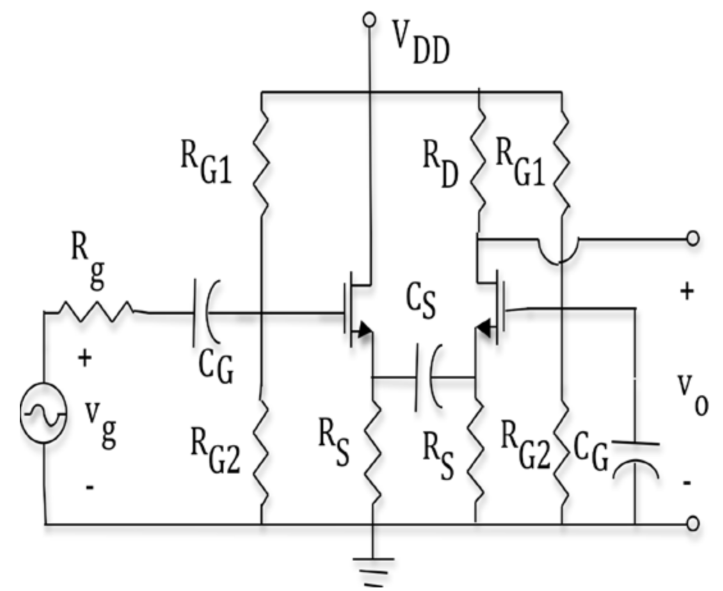
\includegraphics[scale=0.23]{./plots/6.png}
\end{center}
\caption{CD-CG Amplifier}
\end{figure}
\FloatBarrier
\textbf{Experiment}\\
The circuit was breadboarded as designed, and a function generator was connected to the input of the circuit. An oscilloscope was then used to monitor the input and output of the circuit with 10X probes. The input was held at approximately 110 mV, and the frequency was swept from 100 Hz to 3 MHz, hitting in intervals of 100, 300, 1k, 3k and so on for even log spacing for frequency. The values for amplitude were recorded, and the cutoffs determined\\\par
\textbf{Data}\\
Gain was determined as the ratio of output voltage to input at each measured frequency, and then was plotted with log frequency scaling. A dotted line representing half power gain is included, as well as numerical values for cutoffs and midband gain.
\FloatBarrier
\begin{figure}[h!]
\begin{center}
    	\resizebox{0.6\textwidth}{!}{% GNUPLOT: LaTeX picture
\setlength{\unitlength}{0.240900pt}
\ifx\plotpoint\undefined\newsavebox{\plotpoint}\fi
\begin{picture}(1500,900)(0,0)
\sbox{\plotpoint}{\rule[-0.200pt]{0.400pt}{0.400pt}}%
\put(151.0,196.0){\rule[-0.200pt]{4.818pt}{0.400pt}}
\put(131,196){\makebox(0,0)[r]{ 4}}
\put(1419.0,196.0){\rule[-0.200pt]{4.818pt}{0.400pt}}
\put(151.0,282.0){\rule[-0.200pt]{4.818pt}{0.400pt}}
\put(131,282){\makebox(0,0)[r]{ 6}}
\put(1419.0,282.0){\rule[-0.200pt]{4.818pt}{0.400pt}}
\put(151.0,368.0){\rule[-0.200pt]{4.818pt}{0.400pt}}
\put(131,368){\makebox(0,0)[r]{ 8}}
\put(1419.0,368.0){\rule[-0.200pt]{4.818pt}{0.400pt}}
\put(151.0,454.0){\rule[-0.200pt]{4.818pt}{0.400pt}}
\put(131,454){\makebox(0,0)[r]{ 10}}
\put(1419.0,454.0){\rule[-0.200pt]{4.818pt}{0.400pt}}
\put(151.0,540.0){\rule[-0.200pt]{4.818pt}{0.400pt}}
\put(131,540){\makebox(0,0)[r]{ 12}}
\put(1419.0,540.0){\rule[-0.200pt]{4.818pt}{0.400pt}}
\put(151.0,626.0){\rule[-0.200pt]{4.818pt}{0.400pt}}
\put(131,626){\makebox(0,0)[r]{ 14}}
\put(1419.0,626.0){\rule[-0.200pt]{4.818pt}{0.400pt}}
\put(151.0,712.0){\rule[-0.200pt]{4.818pt}{0.400pt}}
\put(131,712){\makebox(0,0)[r]{ 16}}
\put(1419.0,712.0){\rule[-0.200pt]{4.818pt}{0.400pt}}
\put(151.0,131.0){\rule[-0.200pt]{0.400pt}{4.818pt}}
\put(151,90){\makebox(0,0){ $10^2$}}
\put(151.0,756.0){\rule[-0.200pt]{0.400pt}{4.818pt}}
\put(238.0,131.0){\rule[-0.200pt]{0.400pt}{2.409pt}}
\put(238.0,766.0){\rule[-0.200pt]{0.400pt}{2.409pt}}
\put(352.0,131.0){\rule[-0.200pt]{0.400pt}{2.409pt}}
\put(352.0,766.0){\rule[-0.200pt]{0.400pt}{2.409pt}}
\put(411.0,131.0){\rule[-0.200pt]{0.400pt}{2.409pt}}
\put(411.0,766.0){\rule[-0.200pt]{0.400pt}{2.409pt}}
\put(439.0,131.0){\rule[-0.200pt]{0.400pt}{4.818pt}}
\put(439,90){\makebox(0,0){ $10^3$}}
\put(439.0,756.0){\rule[-0.200pt]{0.400pt}{4.818pt}}
\put(525.0,131.0){\rule[-0.200pt]{0.400pt}{2.409pt}}
\put(525.0,766.0){\rule[-0.200pt]{0.400pt}{2.409pt}}
\put(640.0,131.0){\rule[-0.200pt]{0.400pt}{2.409pt}}
\put(640.0,766.0){\rule[-0.200pt]{0.400pt}{2.409pt}}
\put(698.0,131.0){\rule[-0.200pt]{0.400pt}{2.409pt}}
\put(698.0,766.0){\rule[-0.200pt]{0.400pt}{2.409pt}}
\put(726.0,131.0){\rule[-0.200pt]{0.400pt}{4.818pt}}
\put(726,90){\makebox(0,0){ $10^4$}}
\put(726.0,756.0){\rule[-0.200pt]{0.400pt}{4.818pt}}
\put(813.0,131.0){\rule[-0.200pt]{0.400pt}{2.409pt}}
\put(813.0,766.0){\rule[-0.200pt]{0.400pt}{2.409pt}}
\put(927.0,131.0){\rule[-0.200pt]{0.400pt}{2.409pt}}
\put(927.0,766.0){\rule[-0.200pt]{0.400pt}{2.409pt}}
\put(986.0,131.0){\rule[-0.200pt]{0.400pt}{2.409pt}}
\put(986.0,766.0){\rule[-0.200pt]{0.400pt}{2.409pt}}
\put(1014.0,131.0){\rule[-0.200pt]{0.400pt}{4.818pt}}
\put(1014,90){\makebox(0,0){ $10^5$}}
\put(1014.0,756.0){\rule[-0.200pt]{0.400pt}{4.818pt}}
\put(1101.0,131.0){\rule[-0.200pt]{0.400pt}{2.409pt}}
\put(1101.0,766.0){\rule[-0.200pt]{0.400pt}{2.409pt}}
\put(1215.0,131.0){\rule[-0.200pt]{0.400pt}{2.409pt}}
\put(1215.0,766.0){\rule[-0.200pt]{0.400pt}{2.409pt}}
\put(1274.0,131.0){\rule[-0.200pt]{0.400pt}{2.409pt}}
\put(1274.0,766.0){\rule[-0.200pt]{0.400pt}{2.409pt}}
\put(1302.0,131.0){\rule[-0.200pt]{0.400pt}{4.818pt}}
\put(1302,90){\makebox(0,0){ $10^6$}}
\put(1302.0,756.0){\rule[-0.200pt]{0.400pt}{4.818pt}}
\put(1388.0,131.0){\rule[-0.200pt]{0.400pt}{2.409pt}}
\put(1388.0,766.0){\rule[-0.200pt]{0.400pt}{2.409pt}}
\put(151.0,131.0){\rule[-0.200pt]{0.400pt}{155.380pt}}
\put(151.0,131.0){\rule[-0.200pt]{310.279pt}{0.400pt}}
\put(1439.0,131.0){\rule[-0.200pt]{0.400pt}{155.380pt}}
\put(151.0,776.0){\rule[-0.200pt]{310.279pt}{0.400pt}}
\put(30,453){\makebox(0,0){\hspace{-48pt}Gain ($\frac{V}{V}$)}}
\put(795,29){\makebox(0,0){Frequency (Hz)}}
\put(795,838){\makebox(0,0){CD-CG Amplifier Gain vs Frequency}}
\put(151,404){\usebox{\plotpoint}}
\multiput(151.58,404.00)(0.499,0.759){271}{\rule{0.120pt}{0.707pt}}
\multiput(150.17,404.00)(137.000,206.532){2}{\rule{0.400pt}{0.354pt}}
\multiput(288.00,612.58)(1.548,0.498){95}{\rule{1.333pt}{0.120pt}}
\multiput(288.00,611.17)(148.234,49.000){2}{\rule{0.666pt}{0.400pt}}
\multiput(439.00,661.60)(19.929,0.468){5}{\rule{13.800pt}{0.113pt}}
\multiput(439.00,660.17)(108.357,4.000){2}{\rule{6.900pt}{0.400pt}}
\multiput(576.00,663.93)(13.509,-0.482){9}{\rule{10.100pt}{0.116pt}}
\multiput(576.00,664.17)(129.037,-6.000){2}{\rule{5.050pt}{0.400pt}}
\multiput(726.00,659.58)(5.453,0.493){23}{\rule{4.346pt}{0.119pt}}
\multiput(726.00,658.17)(128.979,13.000){2}{\rule{2.173pt}{0.400pt}}
\multiput(1014.00,670.92)(4.670,-0.494){27}{\rule{3.753pt}{0.119pt}}
\multiput(1014.00,671.17)(129.210,-15.000){2}{\rule{1.877pt}{0.400pt}}
\multiput(1151.00,655.92)(0.706,-0.499){211}{\rule{0.664pt}{0.120pt}}
\multiput(1151.00,656.17)(149.621,-107.000){2}{\rule{0.332pt}{0.400pt}}
\multiput(1302.58,546.54)(0.498,-0.919){81}{\rule{0.120pt}{0.833pt}}
\multiput(1301.17,548.27)(42.000,-75.270){2}{\rule{0.400pt}{0.417pt}}
\multiput(1344.58,468.72)(0.499,-1.165){187}{\rule{0.120pt}{1.031pt}}
\multiput(1343.17,470.86)(95.000,-218.861){2}{\rule{0.400pt}{0.515pt}}
\put(864.0,672.0){\rule[-0.200pt]{36.135pt}{0.400pt}}
\put(151,404){\rule{1pt}{1pt}}
\put(288,612){\rule{1pt}{1pt}}
\put(439,661){\rule{1pt}{1pt}}
\put(576,665){\rule{1pt}{1pt}}
\put(726,659){\rule{1pt}{1pt}}
\put(864,672){\rule{1pt}{1pt}}
\put(1014,672){\rule{1pt}{1pt}}
\put(1151,657){\rule{1pt}{1pt}}
\put(1302,550){\rule{1pt}{1pt}}
\put(1344,473){\rule{1pt}{1pt}}
\put(1439,252){\rule{1pt}{1pt}}
\put(151,484){\usebox{\plotpoint}}
\multiput(151,484)(20.756,0.000){63}{\usebox{\plotpoint}}
\put(1439,484){\usebox{\plotpoint}}
\put(151.0,131.0){\rule[-0.200pt]{0.400pt}{155.380pt}}
\put(151.0,131.0){\rule[-0.200pt]{310.279pt}{0.400pt}}
\put(1439.0,131.0){\rule[-0.200pt]{0.400pt}{155.380pt}}
\put(151.0,776.0){\rule[-0.200pt]{310.279pt}{0.400pt}}
\end{picture}
}
\end{center}
\caption{MOS CD-CG Amplifier Frequency Response}
\caption*{$f_L$ = 180 Hz, $f_H$=1.4 MHz, $g_m$ = 15.1}
\end{figure}
\FloatBarrier
\textbf{Conclusions}\\
This amplifier topology offered the best bandwidth, exceeding the cascode design by 2.9x and the CS by nearly 20x. The gain suffered on this design moderately, at 15.1 in the midband, which is approximately half of the cascode. This design works because it takes advantage of the wide bandwidth buffering characteristics of the common drain amplifier to feed the common gate stage, which is essentially unaffected by the Miller Effect. Since both stages are largely immune to effects of frequency response, the bandwidth is extended again. The gain is possibly lower in this design due to losses in the buffering of the input in the first stage, which would lead to an overall lower gain out of the second stage if it has a gain similar to the CS design.

%-----------------------------------------------------------------------------
%	Conclusion
%----------------------------------------------------------------------------------------
\vspace{-12pt}\section{Conclusion}
In this experiment, the design, analysis and testing of the bandwidth and gain behavior of several MOSFET amplifier designs dependent on frequency was performed. It was first observed in a common source amplifier that there is a gain dependence on frequency, such that a pass band called the midband exists in a MOSFET amplifier's frequency response. The cutoff frequencies of several differently loaded CS amplifers were found, and from them the gate capacitance values of a 2N7000 were found to be $C_{gs}$ = -19.9 pF and $C_{gd}$ = 16.8 pF. Better MOSFET amplifier designs were tested in order to obtain a higher bandwidth. First, a cascode based design was built, providing a improvement in bandwidth of about 7x under similar circumstances with better gain. A common-drain-common-gate design was then tested, showing again an improvement on the previous designs, having about 20x the bandwidth performance of the CS and 3x the performance of the cascode. This was afforded mainly by a two stage design in which each stage is largely intolerant to the Miller effect and frequency dependence. The overall outcomes of this experiment were a understanding of how to design high frequency amplifiers, mainly by targeting topologies that minimize the Miller effect and frequency dependence.

\end{document}